\documentclass{article}

\usepackage{graphicx}
\usepackage{tikz}
\usepackage{tikzsymbols}
\usetikzlibrary{calc,patterns,shapes.geometric}
\pagestyle{empty}
\usepackage[margin=0pt]{geometry}
\geometry{papersize={14in,12in}}

\def\centerarc[#1](#2)(#3:#4:#5){\draw[#1] ($(#2)+({#5*cos(#3)},{#5*sin(#3)})$) arc (#3:#4:#5);}

\begin{document}
	\begin{figure}
		\centering
		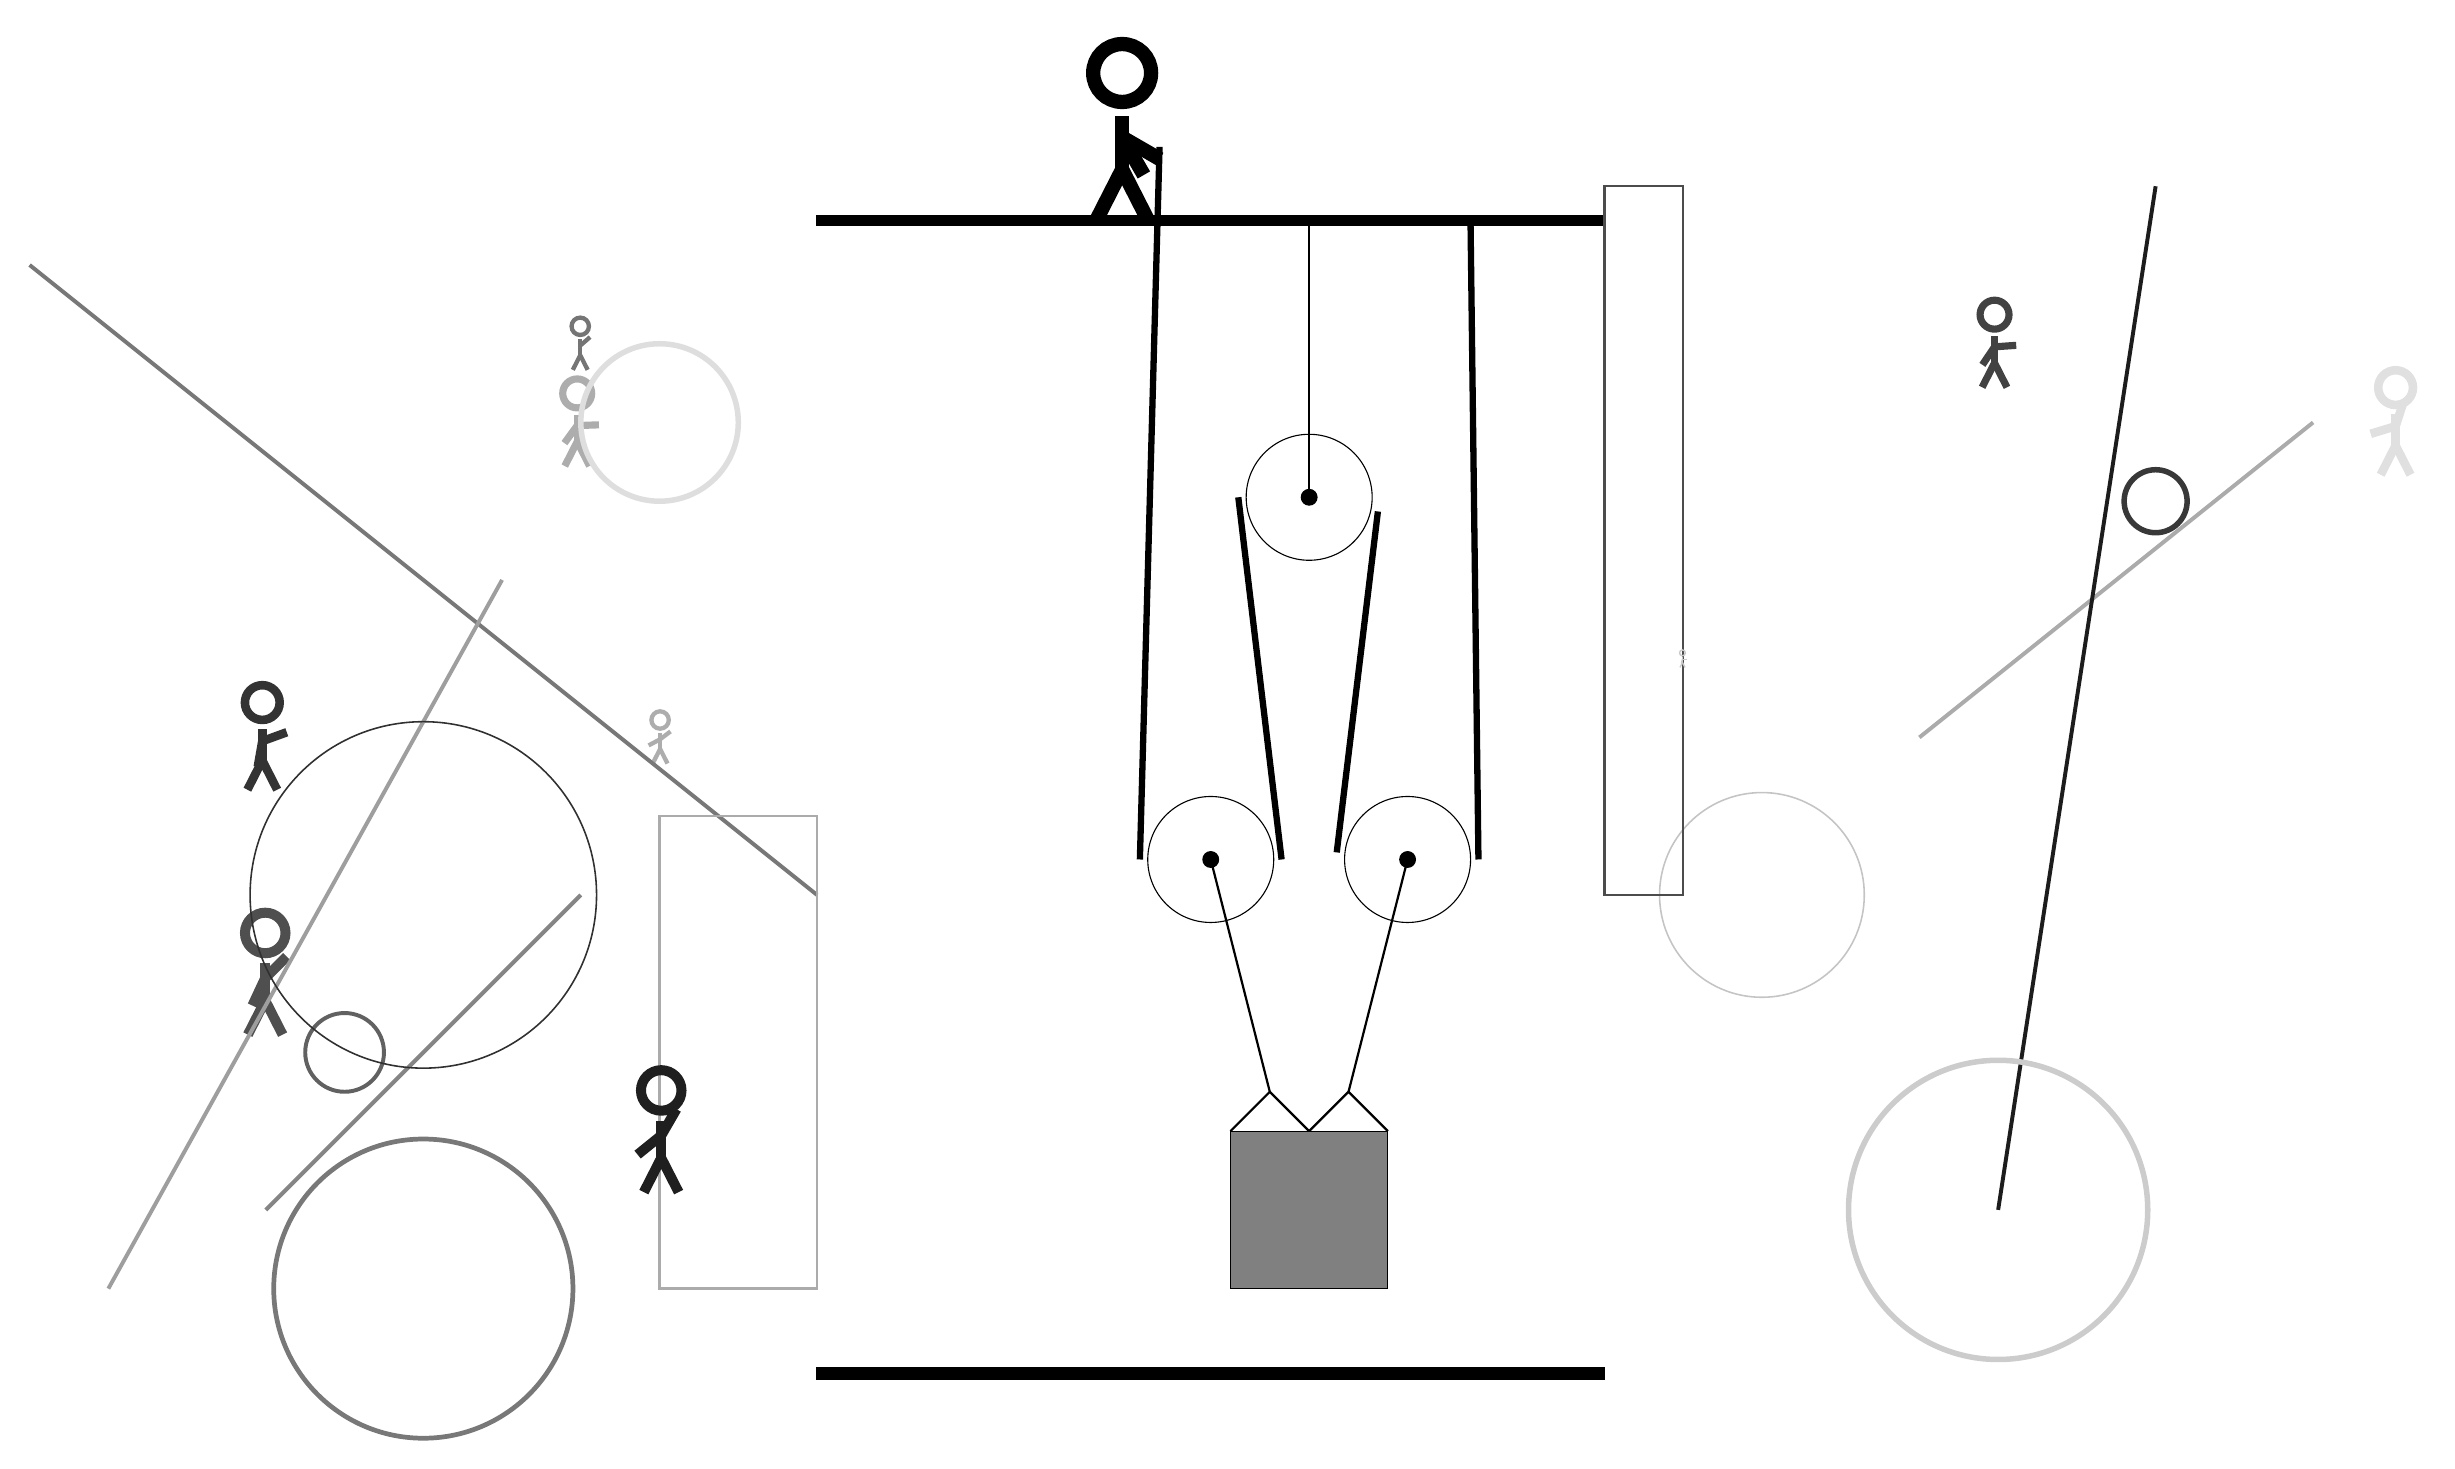
\begin{tikzpicture}
			%%%%% START %%%%%
			
			\draw[fill=black] (-4, 11.5) rectangle (6, 11.625);
			
			\draw (1, 3.45) circle (0.8);
			\draw[fill=black] (1, 3.45) circle (0.1);
			
			\draw (2.25, 8.05) circle (0.8);
			\draw[fill=black] (2.25, 8.05) circle (0.1);
			\draw[thick] (2.25, 8.05) -- (2.25, 11.5);
			
			\draw (3.5, 3.45) circle (0.8);
			\draw[fill=black] (3.5, 3.45) circle (0.1);
			
			\draw[thick] (3.5, 3.45) -- (2.75, 0.5);
			\draw[thick] (1, 3.45) -- (1.75, 0.5);
			\draw[thick]  (1.25, 0) -- (1.75, 0.5) -- (2.25, 0);
			\draw[thick]  (2.25, 0) -- (2.75, 0.5) -- (3.25, 0);
			\draw[fill=black!50] (1.25, 0) rectangle (3.25, -2);
			
			\draw [line width=0.2mm, color=black!23](8, 3) circle (1.3);
			
			\draw[line width=0.5mm, color=black!33](10, 5) -- (15, 9);
			\draw[line width=0.5mm, color=black!48](-7, 3) -- (-11, -1);
			\node[line width=0.4mm, color=black!74] at (11, 10) {\Strichmaxerl[5][56][4]};
			\draw [line width=0.6mm, color=black!53](-9, -2) circle (1.9);
			
			\node[line width=0.7mm, color=black!54] at (-7, 10) {\Strichmaxerl[3][90][41]};
			\node[line width=0.3mm, color=black!80] at (-11, 5) {\Strichmaxerl[6][80][20]};
			\draw[line width=0.5mm, color=black!89](11, -1) -- (13, 12);
			\draw[line width=0.3mm, color=black!70] (6, 3) rectangle (7, 12);
			\node[line width=0.5mm, color=black!32] at (-7, 9) {\Strichmaxerl[5][54][2]};
			\node[line width=0.6mm, color=black!69] at (-11, 2) {\Strichmaxerl[7][65][45]};
			\draw [line width=0.7mm, color=black!78](13, 8) circle (0.4);
			\draw [line width=0.7mm, color=black!20](11, -1) circle (1.9);
			
			\draw [line width=0.5mm, color=black!62](-10, 1) circle (0.5);
			\node[line width=0.3mm, color=black!32] at (-6, 5) {\Strichmaxerl[3][28][37]};
			\draw[line width=0.5mm, color=black!53](-4, 3) -- (-14, 11);
			
			\draw[line width=0.5mm, color=black!38](-8, 7) -- (-13, -2);
			\node[line width=0.7mm, color=black!12] at (16, 9) {\Strichmaxerl[6][17][72]};
			\draw [line width=0.2mm, color=black!81](-9, 3) circle (2.2);
			
			\draw[line width=0.3mm, color=black!33] (-4, 4) rectangle (-6, -2);
			\node[line width=0.6mm, color=black!88] at (-6, 0) {\Strichmaxerl[7][39][60]};
			
			\node[line width=0.5mm, color=black!21] at (7, 6) {\Strichmaxerl[1][76][0]};
			
			\draw [line width=0.7mm, color=black!13](-6, 9) circle (1.0);
			
			\draw[line width=0.8mm] (0.35, 12.5) --  (0.1, 3.45);
			\centerarc[line width=0.8mm](1, 3.45)(180:360:0.9);
			\draw[line width=0.8mm] (1.9, 3.45) -- (1.35, 8.05);
			\centerarc[line width=0.8mm](2.25, 8.05)(-20:180:0.9);
			\draw[line width=0.8mm](3.123, 7.87) -- (2.6, 3.54);
			\centerarc[line width=0.8mm](3.5, 3.45)(160:360:0.9);
			\draw[line width=0.8mm](4.4, 3.45) -- (4.3, 11.5);
			
			\node at (-0.07, 12.7) {\Strichmaxerl[10][120][-30]};
			
			\draw[fill=black] (-4, -3) rectangle (6, -3.15);
			
			%%%%% END %%%%%
		\end{tikzpicture}
	\end{figure}	
\end{document}